\documentclass[letterpaper, 12pt]{article}
\usepackage[english]{babel}
\usepackage[letterpaper,top=2cm,bottom=2cm,left=3cm,right=3cm,marginparwidth=1.75cm]{geometry}
\usepackage[colorlinks=true, allcolors=blue]{hyperref}
\usepackage{graphicx}
\graphicspath{{Figures/}{./}}
\usepackage{amsmath}
\usepackage{amssymb}
\usepackage{amsthm}
\usepackage{indentfirst}
\setlength{\parindent}{20pt}
\usepackage{siunitx}
\usepackage[justification=centering]{caption}
\usepackage{float}
\usepackage{longtable}
\usepackage{tabularray}

\nocite{}

\title{An Investigation of the Moments\\ About a Horizontal Rigid Beam \\ IB Physics SL}
\author{Ethan Chen}

\begin{document}

\maketitle

\begin{center}
    Mr. Shaw
\end{center}

\section{Experimental plan}

\subsection{Manipulated variable}
The manipulated variable is the distance of the weights from the pivot point /\unit{m}.
In this lab, the manipulated variable will be changed by moving the position of the weights to the right.
This change will be measured by the ruler that the weights are hanging from.

\subsection{Responding variable}
The responding variable is the amount of force that the spring balance measures /\unit{N}.
The responding variable will be measured using a spring balance.


\subsection{Controlled variables}

\begin{table}[H]
    \centering
    \begin{tabular}{|l|l|l|}
        \hline
        Condition                                                                                                  & How to control it                                                                                                                                                            & Why it must be controlled                                                                                                                                                                                                                                                           \\
        \hline
        \begin{tabular}[c]{@{}l@{}}The position\\of the pivot\\and spring \\balance\\along the ruler.\end{tabular} & \begin{tabular}[c]{@{}l@{}}Recording each\\trial with the pivot\\and the spring\\balance consistently\\positioned at the exact\\same location along\\the ruler.\end{tabular} & \begin{tabular}[c]{@{}l@{}}Varying the position\\of these objects will\\change the distances\\between the pivot to\\the ruler's center of\\mass, the weights,\\and the spring balance.\\This will ultimately\\cause inconsistencies\\in the calculated torque\\values.\end{tabular} \\
        \hline
        \begin{tabular}[c]{@{}l@{}}The number\\of weights\\suspended on\\the ruler.\end{tabular}                   & \begin{tabular}[c]{@{}l@{}}Recording each trial\\with the same number\\of weights\\suspended from\\the ruler.\end{tabular}                                                   & \begin{tabular}[c]{@{}l@{}}Varying the number\\of weights suspended\\on the ruler will cause\\the gravitational force\\of the weights\\to vary, affecting\\both calculations\\for net force and\\calculations\\for net torque.\end{tabular}                                         \\
        \hline
    \end{tabular}
    \caption{Controlled variables in the experiment}
    \label{table:controlled_variables}
\end{table}


\section{Background Information}

\subsection{Horizontal ruler requirement}

If this experiment is to be physically conducted, then there is a need for the
ruler or beam to be horizontal. This is because the torques acting on the beam only come from the the force
component perpendicular to the beam, therefore using a horizontal beam would
then simplify the analysis, as the calculation of the components of
the forces perpendicular to the beam would not be required.

What is meant by the beam/ruler to be horizontal is visually shown by the ruler in
Figure \ref*{fig:horizontal}.

\begin{figure}[H]
    \centering
    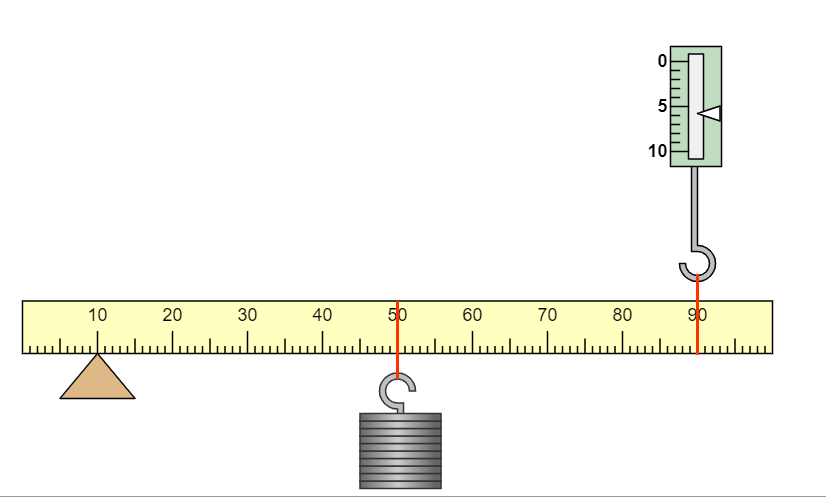
\includegraphics[width=0.65\textwidth]{horizontal}
    \caption{Horizontal beam/ruler in the apparatus of the investigation.}
    \label{fig:horizontal}
\end{figure}

\subsection{Conditions for static equilibrium and derivations of required equations}

The following conditions need to be met for static equilibrium:
\begin{itemize}
    \item The sum of all forces acting on the system must be equal to zero ($\sum F = 0$).
    \item The sum of all torques with respect to some point in the system must be equal to zero ($\sum \tau = 0$).
\end{itemize}


\begin{figure}[H]
    \centering
    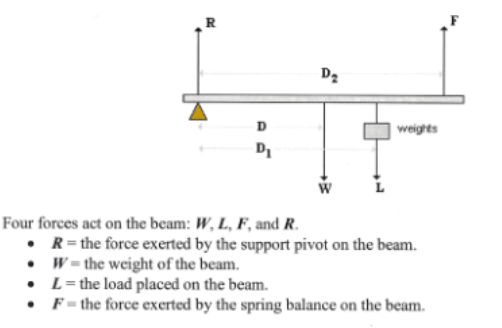
\includegraphics[width=0.65\textwidth]{labelled apparatus and variables}
    \caption{Apparatus labelled with variables along with descriptions of forces acting in the system}
    \label{fig:labapparatus}
\end{figure}

With reference to the variables in Figure \ref*{fig:labapparatus}, we can derive the following equations.

\subsubsection*{Forces acting on the beam}
\begin{align*}
     & \sum F                      = 0
    \\
     & \vec{R} + \vec{L} + \vec{F} = 0
\end{align*}

\subsubsection*{Torques acting on the beam relative to support pivot (orange triangle in Figure \ref*{fig:labapparatus})}

\begin{align*}
     & \text{Assigning clockwise spin as the positive direction}
    \\
     & \sum \tau = 0
    \\
     & \left(\left|\vec{W}\right|\cdot D\right) + \left(\left|\vec{L}\right|\cdot D_1\right) - \left(\left|\vec{F}\right|\cdot D_2\right) = 0
\end{align*}

\section{Raw data}

\subsection{Determination of uncertainty in force measured by spring balance}

Setting the weights the 0.801\unit{m} along the ruler, as shown in Figure
\ref*{fig:uncRef}, the range of the force measured by the spring balance is
0.5\unit{N}, with a minimum value of 9.2\unit{N} and a maximum value of
9.7\unit{N}.

\begin{figure}[H]
    \centering
    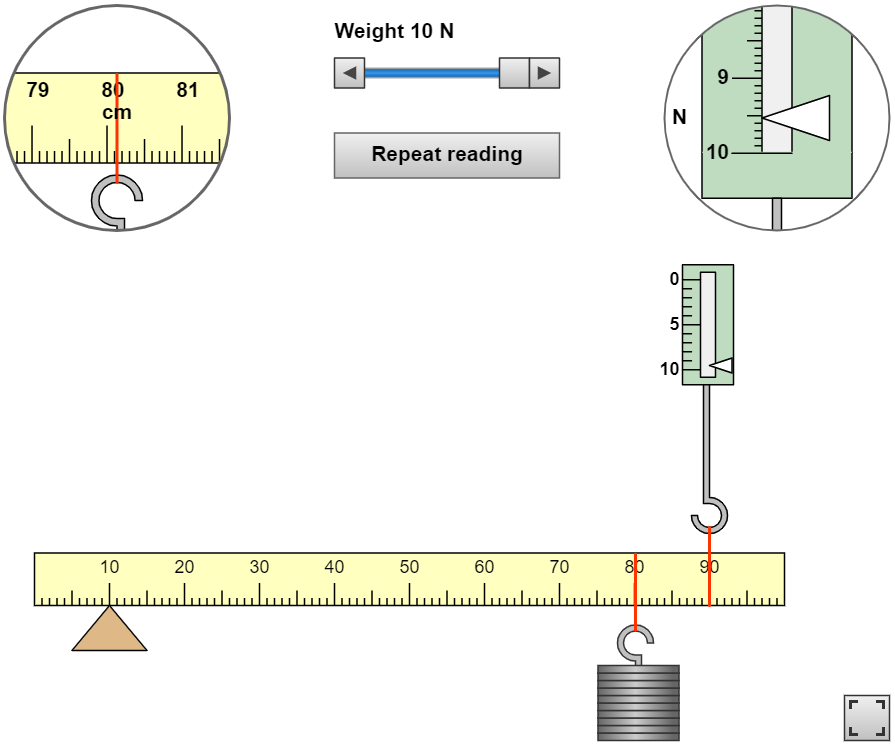
\includegraphics[width=0.65\textwidth]{uncRef}
    \caption{Positioning of weight in apparatus for uncertainty calculation of spring balance}
    \label{fig:uncRef}
\end{figure}

Therefore, by dividing this range by 2, the uncertainty of the force probe is
determined to be 0.3\unit{N}.

\subsection{Collected raw data}


\begin{longtable}{|c|c|}
    \caption{Table of Position of weights along ruler with respective values of Force measured by spring scale}                                                                                                                                                                                                                                                          \\
    \hline
    \multicolumn{1}{|l|}{\begin{tabular}[c]{@{}l@{}}Position of weights\\along ruler /\unit{m}\\($\Delta \unit{m} \pm 0.001\unit{m}$)\end{tabular}} & \multicolumn{1}{l|}{\begin{tabular}[c]{@{}l@{}}Force measured by\\spring scale /\unit{N}\\($\Delta \unit{m} \pm 0.5\unit{N}$)\end{tabular}}  \endfirsthead
    \hline
    $0.200$                                                                                                                                                                     & $2.0$                                                                                                                                                                                  \\
    \hline
    $0.210$                                                                                                                                                                     & $2.1$                                                                                                                                                                                  \\
    \hline
    $0.220$                                                                                                                                                                     & $2.3$                                                                                                                                                                                  \\
    \hline
    $0.230$                                                                                                                                                                     & $2.4$                                                                                                                                                                                  \\
    \hline
    $0.240$                                                                                                                                                                     & $2.5$                                                                                                                                                                                  \\
    \hline
    $0.250$                                                                                                                                                                     & $2.6$                                                                                                                                                                                  \\
    \hline
    $0.260$                                                                                                                                                                     & $2.8$                                                                                                                                                                                  \\
    \hline
    $0.270$                                                                                                                                                                     & $2.9$                                                                                                                                                                                  \\
    \hline
    $0.280$                                                                                                                                                                     & $3.0$                                                                                                                                                                                  \\
    \hline
    $0.290$                                                                                                                                                                     & $3.1$                                                                                                                                                                                  \\
    \hline
    $0.300$                                                                                                                                                                     & $3.2$                                                                                                                                                                                  \\
    \hline
    $0.310$                                                                                                                                                                     & $3.4$                                                                                                                                                                                  \\
    \hline
    $0.320$                                                                                                                                                                     & $3.5$                                                                                                                                                                                  \\
    \hline
    $0.330$                                                                                                                                                                     & $3.6$                                                                                                                                                                                  \\
    \hline
    $0.340$                                                                                                                                                                     & $3.8$                                                                                                                                                                                  \\
    \hline
    $0.350$                                                                                                                                                                     & $3.9$                                                                                                                                                                                  \\
    \hline
    $0.360$                                                                                                                                                                     & $4.0$                                                                                                                                                                                  \\
    \hline
    $0.370$                                                                                                                                                                     & $4.2$                                                                                                                                                                                  \\
    \hline
    $0.380$                                                                                                                                                                     & $4.3$                                                                                                                                                                                  \\
    \hline
    $0.390$                                                                                                                                                                     & $4.4$                                                                                                                                                                                  \\
    \hline
    $0.400$                                                                                                                                                                     & $4.5$                                                                                                                                                                                  \\
    \hline
    $0.410$                                                                                                                                                                     & $4.6$                                                                                                                                                                                  \\
    \hline
    $0.420$                                                                                                                                                                     & $4.8$                                                                                                                                                                                  \\
    \hline
    $0.430$                                                                                                                                                                     & $4.9$                                                                                                                                                                                  \\
    \hline
    $0.440$                                                                                                                                                                     & $5.0$                                                                                                                                                                                  \\
    \hline
    $0.450$                                                                                                                                                                     & $5.2$                                                                                                                                                                                  \\
    \hline
    $0.460$                                                                                                                                                                     & $5.2$                                                                                                                                                                                  \\
    \hline
    $0.470$                                                                                                                                                                     & $5.4$                                                                                                                                                                                  \\
    \hline
    $0.480$                                                                                                                                                                     & $5.5$                                                                                                                                                                                  \\
    \hline
    $0.490$                                                                                                                                                                     & $5.6$                                                                                                                                                                                  \\
    \hline
    $0.500$                                                                                                                                                                     & $5.8$                                                                                                                                                                                  \\
    \hline
    $0.510$                                                                                                                                                                     & $5.9$                                                                                                                                                                                  \\
    \hline
    $0.520$                                                                                                                                                                     & $6.0$                                                                                                                                                                                  \\
    \hline
    $0.530$                                                                                                                                                                     & $6.2$                                                                                                                                                                                  \\
    \hline
    $0.540$                                                                                                                                                                     & $6.3$                                                                                                                                                                                  \\
    \hline
    $0.550$                                                                                                                                                                     & $6.5$                                                                                                                                                                                  \\
    \hline
    $0.560$                                                                                                                                                                     & $6.7$                                                                                                                                                                                  \\
    \hline
    $0.570$                                                                                                                                                                     & $6.6$                                                                                                                                                                                  \\
    \hline
    $0.580$                                                                                                                                                                     & $6.8$                                                                                                                                                                                  \\
    \hline
    $0.590$                                                                                                                                                                     & $6.8$                                                                                                                                                                                  \\
    \hline
    $0.600$                                                                                                                                                                     & $7.1$                                                                                                                                                                                  \\
    \hline
    $0.610$                                                                                                                                                                     & $7.2$                                                                                                                                                                                  \\
    \hline
    $0.620$                                                                                                                                                                     & $7.3$                                                                                                                                                                                  \\
    \hline
    $0.630$                                                                                                                                                                     & $7.4$                                                                                                                                                                                  \\
    \hline
    $0.640$                                                                                                                                                                     & $7.6$                                                                                                                                                                                  \\
    \hline
    $0.650$                                                                                                                                                                     & $7.7$                                                                                                                                                                                  \\
    \hline
    $0.660$                                                                                                                                                                     & $7.8$                                                                                                                                                                                  \\
    \hline
    $0.670$                                                                                                                                                                     & $7.9$                                                                                                                                                                                  \\
    \hline
    $0.680$                                                                                                                                                                     & $8.0$                                                                                                                                                                                  \\
    \hline
    $0.690$                                                                                                                                                                     & $8.2$                                                                                                                                                                                  \\
    \hline
    $0.700$                                                                                                                                                                     & $8.3$                                                                                                                                                                                  \\
    \hline
    $0.710$                                                                                                                                                                     & $8.4$                                                                                                                                                                                  \\
    \hline
    $0.720$                                                                                                                                                                     & $8.6$                                                                                                                                                                                  \\
    \hline
    $0.730$                                                                                                                                                                     & $8.7$                                                                                                                                                                                  \\
    \hline
    $0.740$                                                                                                                                                                     & $8.8$                                                                                                                                                                                  \\
    \hline
    $0.750$                                                                                                                                                                     & $8.9$                                                                                                                                                                                  \\
    \hline
    $0.760$                                                                                                                                                                     & $9.1$                                                                                                                                                                                  \\
    \hline
    $0.770$                                                                                                                                                                     & $9.2$                                                                                                                                                                                  \\
    \hline
    $0.780$                                                                                                                                                                     & $9.3$                                                                                                                                                                                  \\
    \hline
    $0.790$                                                                                                                                                                     & $9.5$                                                                                                                                                                                  \\
    \hline
    $0.800$                                                                                                                                                                     & $9.6$                                                                                                                                                                                  \\
    \hline
    $0.810$                                                                                                                                                                     & $9.7$                                                                                                                                                                                  \\
    \hline
    $0.820$                                                                                                                                                                     & $9.8$                                                                                                                                                                                  \\
    \hline
    $0.830$                                                                                                                                                                     & $10.0$                                                                                                                                                                                 \\
    \hline
\end{longtable}


\section{Processed data}

Taking the trial with the weight positioned at $0.200\unit{m}$ along the ruler,
we can determine the predicted force of the spring balance for this trial.

Because the force applied by the pivot point is unknown but the weight of the ruler is known (1.5\unit{N}),
then only the torque equation defined earlier (shown below) can be used to solve for
the predicted force of the spring balance.
$$
    \left(\left|\vec{W}\right|\cdot D\right) + \left(\left|\vec{L}\right|\cdot D_1\right) - \left(\left|\vec{F}\right|\cdot D_2\right) = 0
$$

\begin{figure}[H]
    \centering
    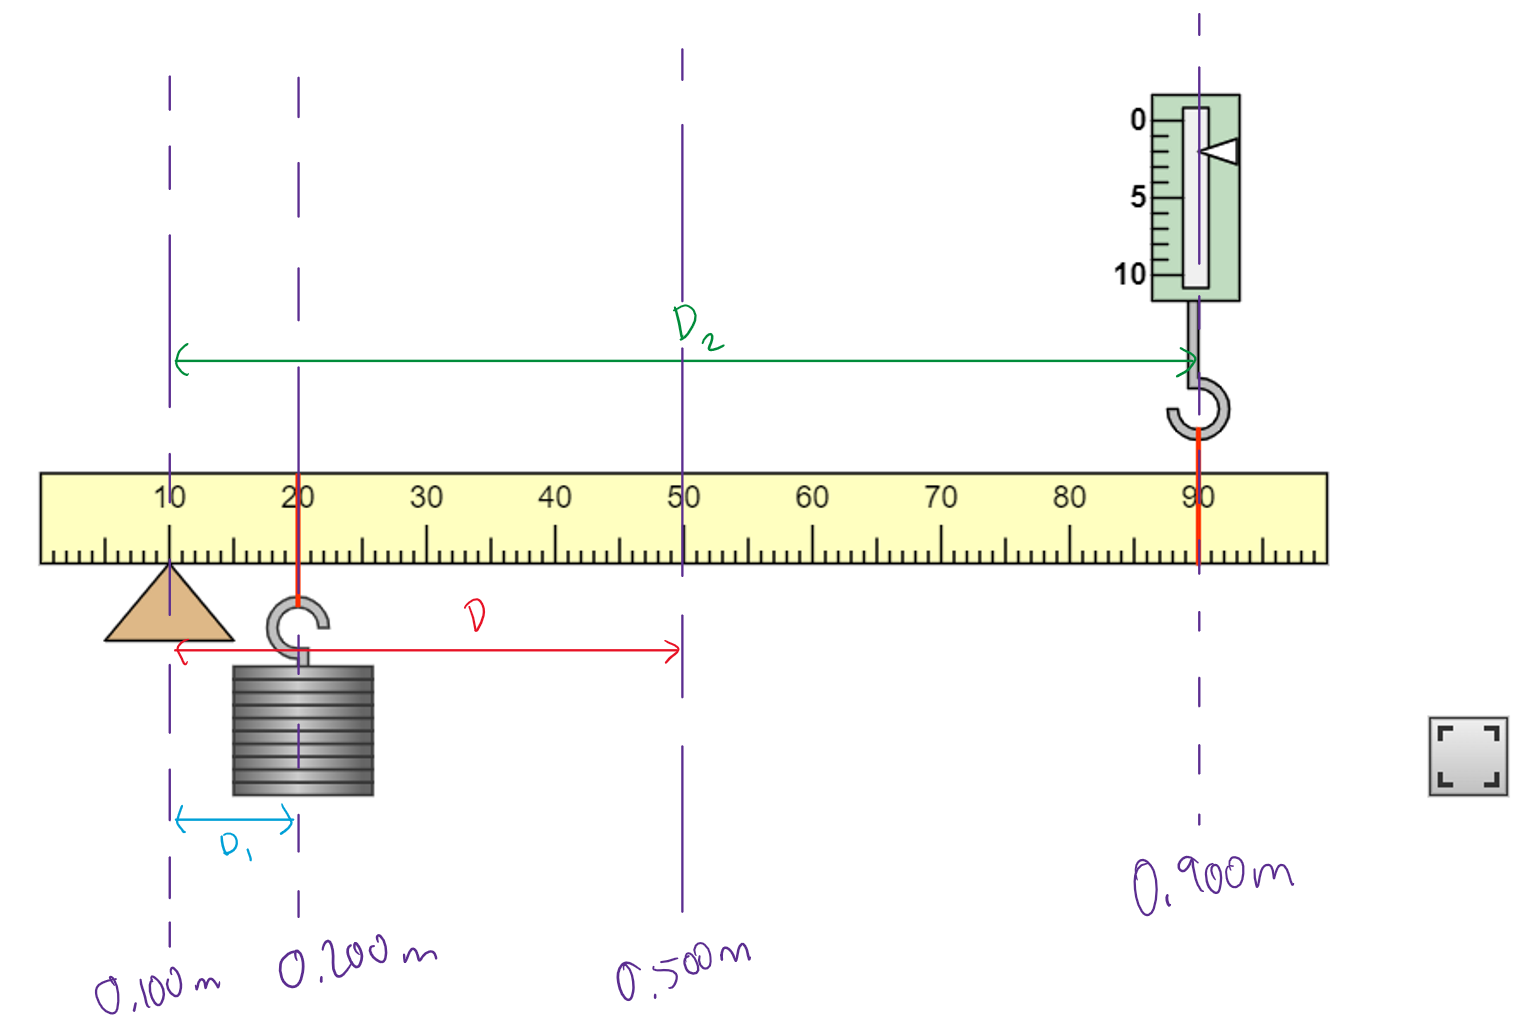
\includegraphics[width=0.65\textwidth]{distanceref}
    \caption{Reference for distance and positions of objects along ruler}
    \label{fig:distRef}
\end{figure}

The calculation for the predicated force of the spring balance given that
the weight is positioned at $0.200\unit{m}$ along the ruler is shown below,
with distance values originating from Figure \ref*{fig:distRef}

\begin{align*}
     & \left(\left|\vec{W}\right|\cdot D\right) + \left(\left|\vec{L}\right|\cdot D_1\right) - \left(\left|\vec{F}\right|\cdot D_2\right) = 0
\end{align*}

\begin{align*}
    \text{where } & \left|\vec{W}\right| = \text{ the magnitude of the weight of the ruler } /\unit{N}
    \\
                  & \left|\vec{L}\right| = \text{ the magnitude of the weight of the weights suspended on the ruler } /\unit{N}
    \\
                  & \left|\vec{F}\right| = \text{ the magnitude of the force applied onto the ruler by the}
    \\ &\text{ spring balance } /\unit{N}
    \\
                  & D = \text{ the distance between the pivot and the ruler's centre of mass } /\unit{m}
    \\ & D_1 = \text{ the distance between the pivot point and the weights } /\unit{m}
    \\ & D_2 = \text{ the distance between the pivot point and the spring balance } /\unit{m}
\end{align*}

\begin{align*}
    \\
                       & \left(\left|\vec{F}\right|\cdot D_2\right) = \left(\left|\vec{W}\right|\cdot D\right) + \left(\left|\vec{L}\right|\cdot D_1\right)
    \\
    \text{Given that } & \left|\vec{W}\right| = 1.5\unit{N}
    \\
                       & \left|\vec{L}\right| = 10\unit{N}
    \\
                       & D_2 = 0.900\unit{m} - 0.100\unit{m} = 0.800\unit{m}
    \\
                       & D = 0.500\unit{m} - 0.100\unit{m} = 0.400\unit{m}
    \\
                       & D_1 = 0.200\unit{m} - 0.100\unit{m} = 0.100\unit{m}
    \\
                       & (0.800\unit{m})\cdot \left|\vec{F}\right| = (0.400\unit{m})(1.5\unit{N}) + (0.100\unit{m})(10\unit{N})
    \\
                       & \left|\vec{F}\right| = 2.0\unit{N}
\end{align*}

Continuing with these calculations, the graph in Figure \ref*{fig:predGraph} shows the
trend of the predicted force of the spring balance with respect to the distance
between the weights and the pivot point.

\begin{figure}[H]
    \centering
    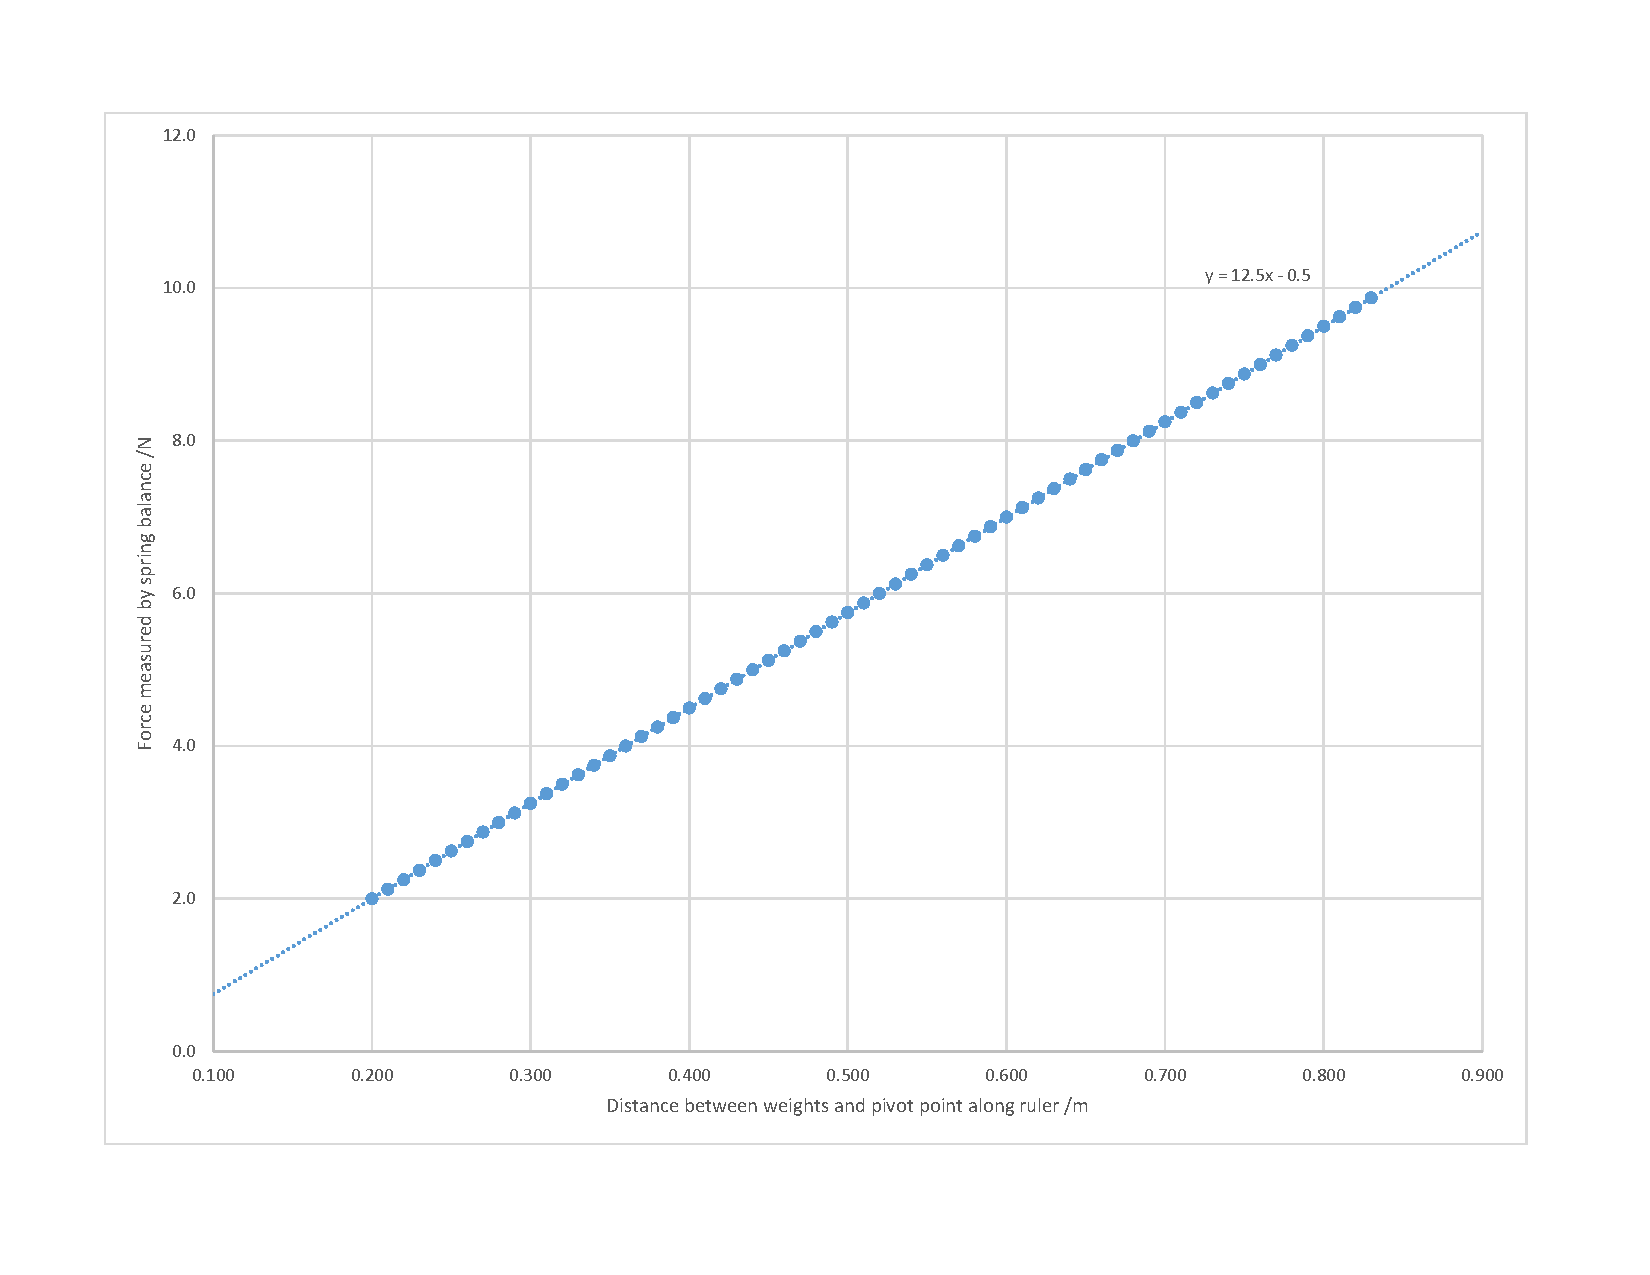
\includegraphics[width=\textwidth]{predictedGraph.pdf}
    \caption{Force measured by spring balance /\unit{N} versus Distance between weights and pivot point along ruler /\unit{m}}
    \label{fig:predGraph}
\end{figure}


\section{Analysis}

\end{document}